\chapter{Experiment}
\label{exp}
\begin{multicols*}{2}

	\section{Introduction}
	\label{exp:intro}
		% TODO - Here I will give a brief overview of the experiments that I will have conducted, the variations that they have between them, and why I chose those variations.
		% So talk about the two experiment types that took place,
		% and how you will analyse first the overarching differences between standard Euclidean geometry and non-Euclidean geometry,
		% And then talk about the differences between the participants results when comparing which scene they viewed first

		% REMEMBER TO SPEAK ABOUT THE MATHS

	\section{Experiments}
	\label{exp:exp}

		\subsection{Standard Euclidean Geometry}
		\label{exp:exp:standard}

			% Talk about the results specific to the standard euclidean geometery here.
			% Used to get a base result for immersion
			% Consistent high ratings for immersion
			% Navigation comfort was varied, but talk about the high mean values

			\end{multicols*}
			\begin{figure}
				\label{exp:fig:standard_immersion}
				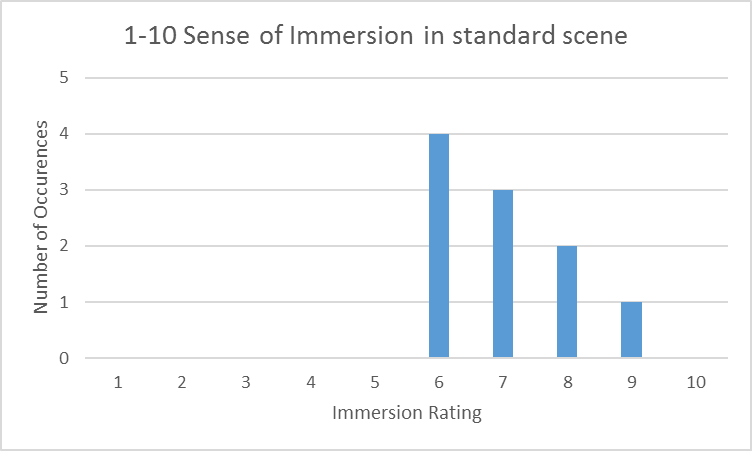
\includegraphics[width=0.7\textwidth]{Images/Standard_Immersion}
				\centering
				\caption{Immersion rating in standard geometry test scene}
			\end{figure}

			\begin{figure}
				\label{exp:fig:standard_comfort}
				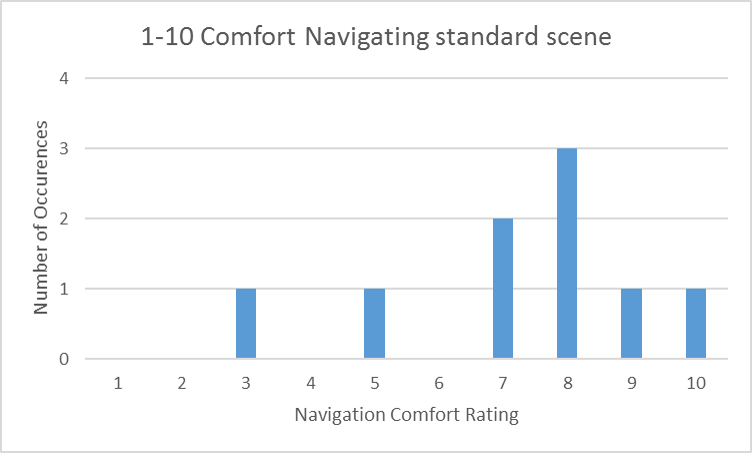
\includegraphics[width=0.7\textwidth]{Images/Standard_Comfort}
				\centering
				\caption{Navigation Comfort rating in standard geometry test scene}
			\end{figure}

			\begin{figure}
				\label{exp:fig:standard_relation}
				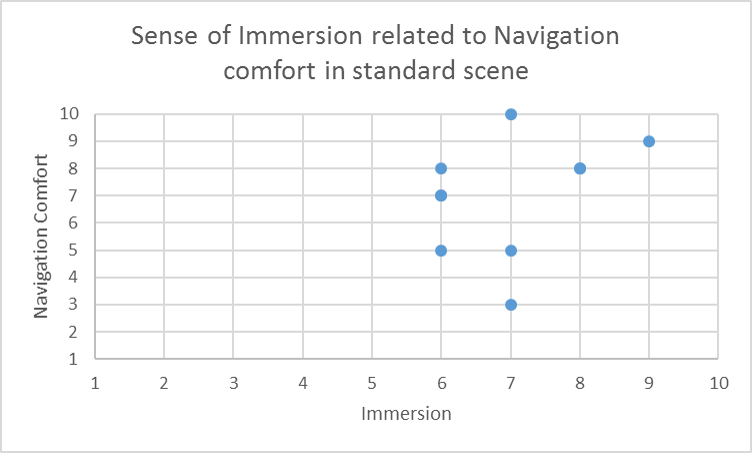
\includegraphics[width=0.7\textwidth]{Images/Standard_Relation}
				\centering
				\caption{Relation between sense of immersion and navigation comfort in standard geometry test scene}
			\end{figure}
			\begin{multicols*}{2}

		\subsection{Non-Euclidean Geometry}
		\label{exp:exp:ne}

			% Talk about the results specific to the non-eucldean geometry here
			% More varied results
			% Same Mean
			% More responses in the higher end of the scale - talk about the written feedback
			% Lower comfort with navigation

			\end{multicols*}
			\begin{figure}
				\label{exp:fig:ne_immersion}
				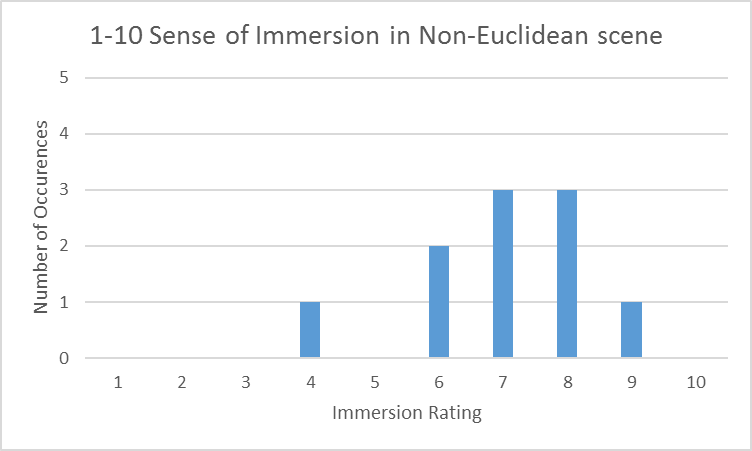
\includegraphics[width=0.7\textwidth]{Images/NE_Immersion}
				\centering
				\caption{Immersion rating in Non-Euclidean geometry test scene}
			\end{figure}

			\begin{figure}
				\label{exp:fig:ne_comfort}
				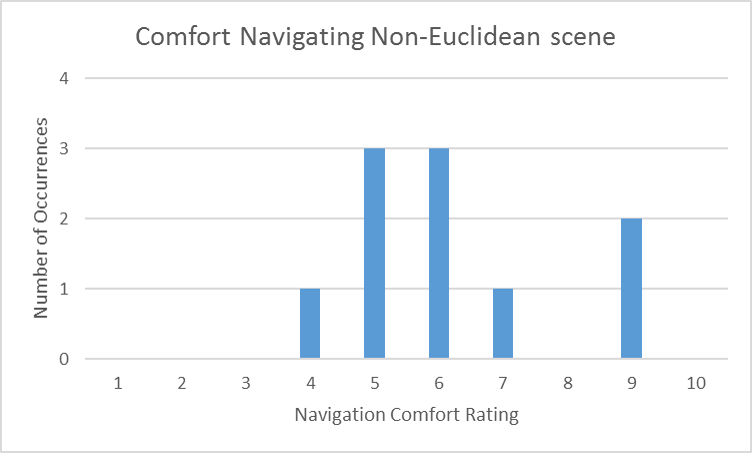
\includegraphics[width=0.7\textwidth]{Images/NE_Comfort}
				\centering
				\caption{Navigation Comfort rating in Non-Euclidean geometry test scene}
			\end{figure}

			\begin{figure}
				\label{exp:fig:ne_relation}
				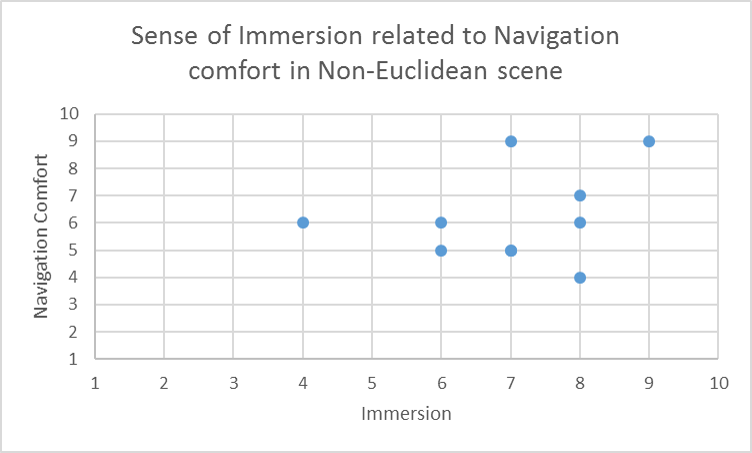
\includegraphics[width=0.7\textwidth]{Images/NE_Relation}
				\centering
				\caption{Relation between sense of immersion and navigation comfort in Non-Euclidean geometry test scene}
			\end{figure}
			\begin{multicols*}{2}

		\subsection{Comparisons}
		\label{exp:exp:comp}

			% Experiment 1 was Standard First
			% Experiment 2 was NE First
			% Talk about the comparisons
			% Talk about how the data MEANs something
			% Participants from exp1 never felt that NE was less immersive, either as immersive or more - quote feedback
			% Participants from exp2 varied a lot more, sometimes NE was more immersive, sometimes  the same, sometimes less so.

			\end{multicols*}
			\begin{figure}
				\label{exp:fig:compare_immersion_exp1}
				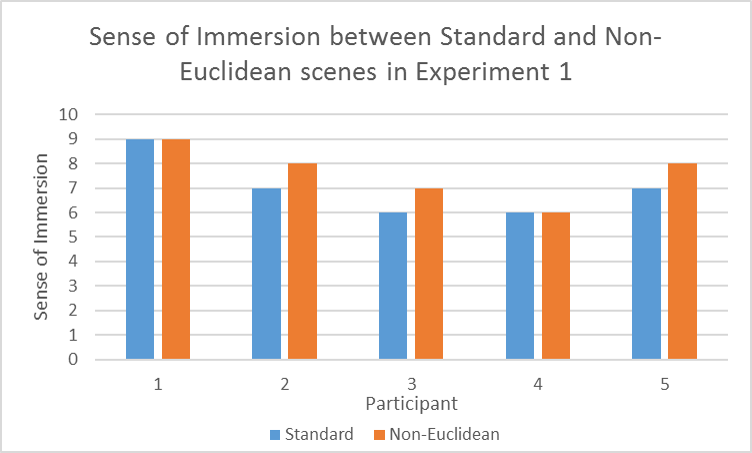
\includegraphics[width=0.7\textwidth]{Images/Compare_Immersion_Exp_1}
				\centering
				\caption{Comparison of participants sense of immersion in the two test scenes, from Experiment 1}
			\end{figure}

			\begin{figure}
				\label{exp:fig:compare_immersion_exp2}
				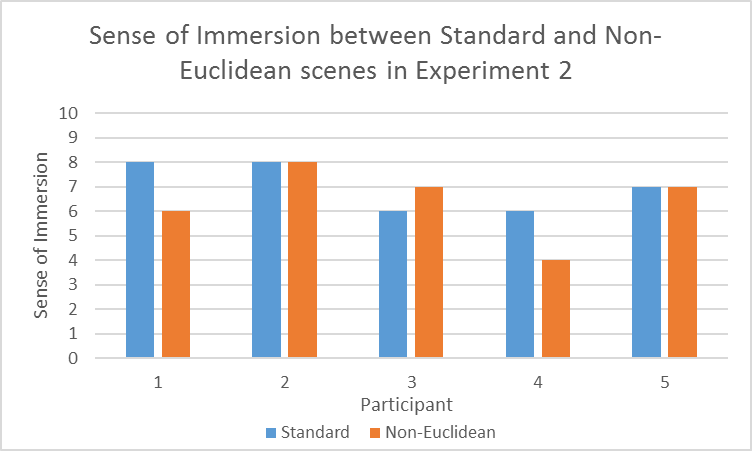
\includegraphics[width=0.7\textwidth]{Images/Compare_Immersion_Exp_2}
				\centering
				\caption{Comparison of participants sense of immersion in the two test scenes, from Experiment 2}
			\end{figure}

			\begin{figure}
				\label{exp:fig:compare_immersion_variation}
				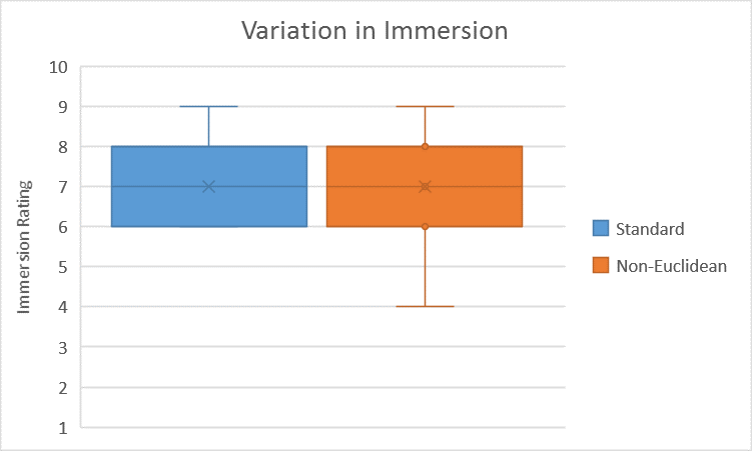
\includegraphics[width=0.7\textwidth]{Images/Compare_Immersion_Variation}
				\centering
				\caption{Mean values, and variation of Range for Immersion in the two test scenes}
			\end{figure}
			\begin{multicols*}{2}

	\section{Summary}
	\label{exp:summary}
		% TODO - Here I will be evaluating the results of the experiments, covering any trends that appeared between the various experiments, discussing potential impacts from the results, as well as covering any additional notes that were provided about the experiments from the participants which weren't directly related to the specific experiment they were part of.

		% Results show that an NE environment can be more immersive than a standard env, so long as the user has had a chance to familiarise themselves in a standard euclid setting first
		% More work needs doing to improve upon the navigation side, there were mixed reviews from both scenes and experiments - quote feedback - room for further study

\end{multicols*}
